% !TEX program = xelatex
\documentclass[12pt]{article}
\usepackage[margin=1in]{geometry}
\usepackage{nopageno} % no page numbers
\usepackage{setspace} \doublespacing

\usepackage{graphicx}
\graphicspath{ {./graphics/} }
\usepackage[dvipsnames]{xcolor}
\definecolor{CrispBlue}{HTML}{0176AE}

\usepackage{fontspec}
\usepackage{tcolorbox}
\usepackage{etoolbox}
\BeforeBeginEnvironment{verbatim*}{\begin{tcolorbox}[colback=CrispBlue!5!white,colframe=CrispBlue!75!black]}%
\AfterEndEnvironment{verbatim*}{\end{tcolorbox}}%

\usepackage{hyperref}
\hypersetup{
    colorlinks,
    citecolor=black,
    filecolor=black,
    linkcolor=black,
    urlcolor=black
}

\renewcommand{\footnotesize}{\fontsize{8pt}{10pt}\selectfont}


\usepackage[labelfont={small,sc,bf},textfont={small,sc,bf}]{caption}
\setlength{\parindent}{24pt}
% \setlength{\parskip}{1em}

\usepackage{tocloft}
\renewcommand{\cftpartleader}{\cftdotfill{\cftdotsep}}
\renewcommand{\cftsecleader}{\cftdotfill{\cftdotsep}}

\usepackage[shortlabels]{enumitem}

\usepackage{lastpage}
\usepackage{fancyhdr}
\pagestyle{fancy}
\fancyhf{}
\renewcommand{\headrulewidth}{0pt}
\rfoot{Page \thepage\ of \pageref*{LastPage}}

\usepackage{amsmath,amsfonts,amssymb}
\usepackage{bm}
\usepackage{mathtools}

\renewcommand{\listfigurename}{List of Figures}

\begin{document}
\setmainfont{SF Pro Text}
\setsansfont{SF Pro Text}
\setmonofont{SF Mono}
\renewcommand{\familydefault}{\sfdefault}

\hypersetup{
    linkcolor=CrispBlue,
    urlcolor=CrispBlue,
    breaklinks=true
}

\noindent David Kirby\\
ECE 529: Introduction to Technical Cybersecurity\\
Spring, 2022
\begin{center}
    \large\bfseries Binary Analysis
\end{center}

Binary analysis can tell us an incredible amount of details about a program. Even though this executable was compiled for x86, using Hopper, I was able to open the \texttt{msg} executable directly, without having to disassemble the code first. From there I was able to see that the first string was hard-coded in the \texttt{main()} program -- string 1: \textbf{\texttt{fubar}} (see Figure~\ref{fig:string1}).
\begin{figure}[!ht]
    \centering
    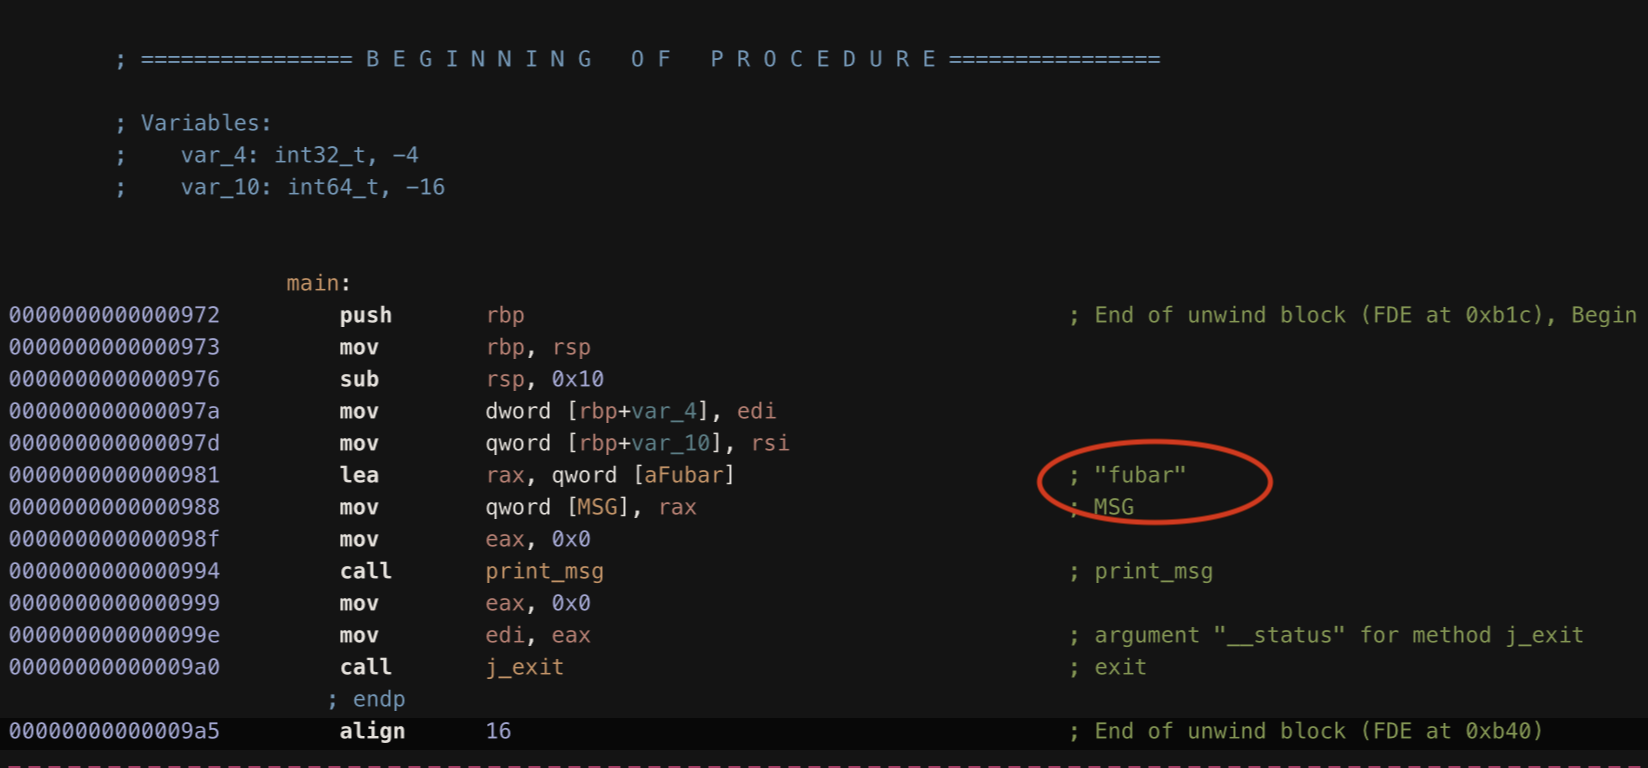
\includegraphics[width=\textwidth]{figure01.png}%\vspace{-1em}
    \caption{String 1 -- fubar.}
    \label{fig:string1}
\end{figure}

To run the executable, I needed to use the x86 Docker container I created for Module 3 of this course. The second string was generated when the program was executed with the shell command uname -- string 2: \textbf{\texttt{Linux}} (see Figure~\ref{fig:string2}). The third string was discovered by setting break points after the operations were performed -- string 3: \textbf{\texttt{J<,4*}}. Finally, the fourth string was revealed after running the program -- string 4: \textbf{\texttt{SE5=3}}.

\begin{figure}[!ht]
    \centering
    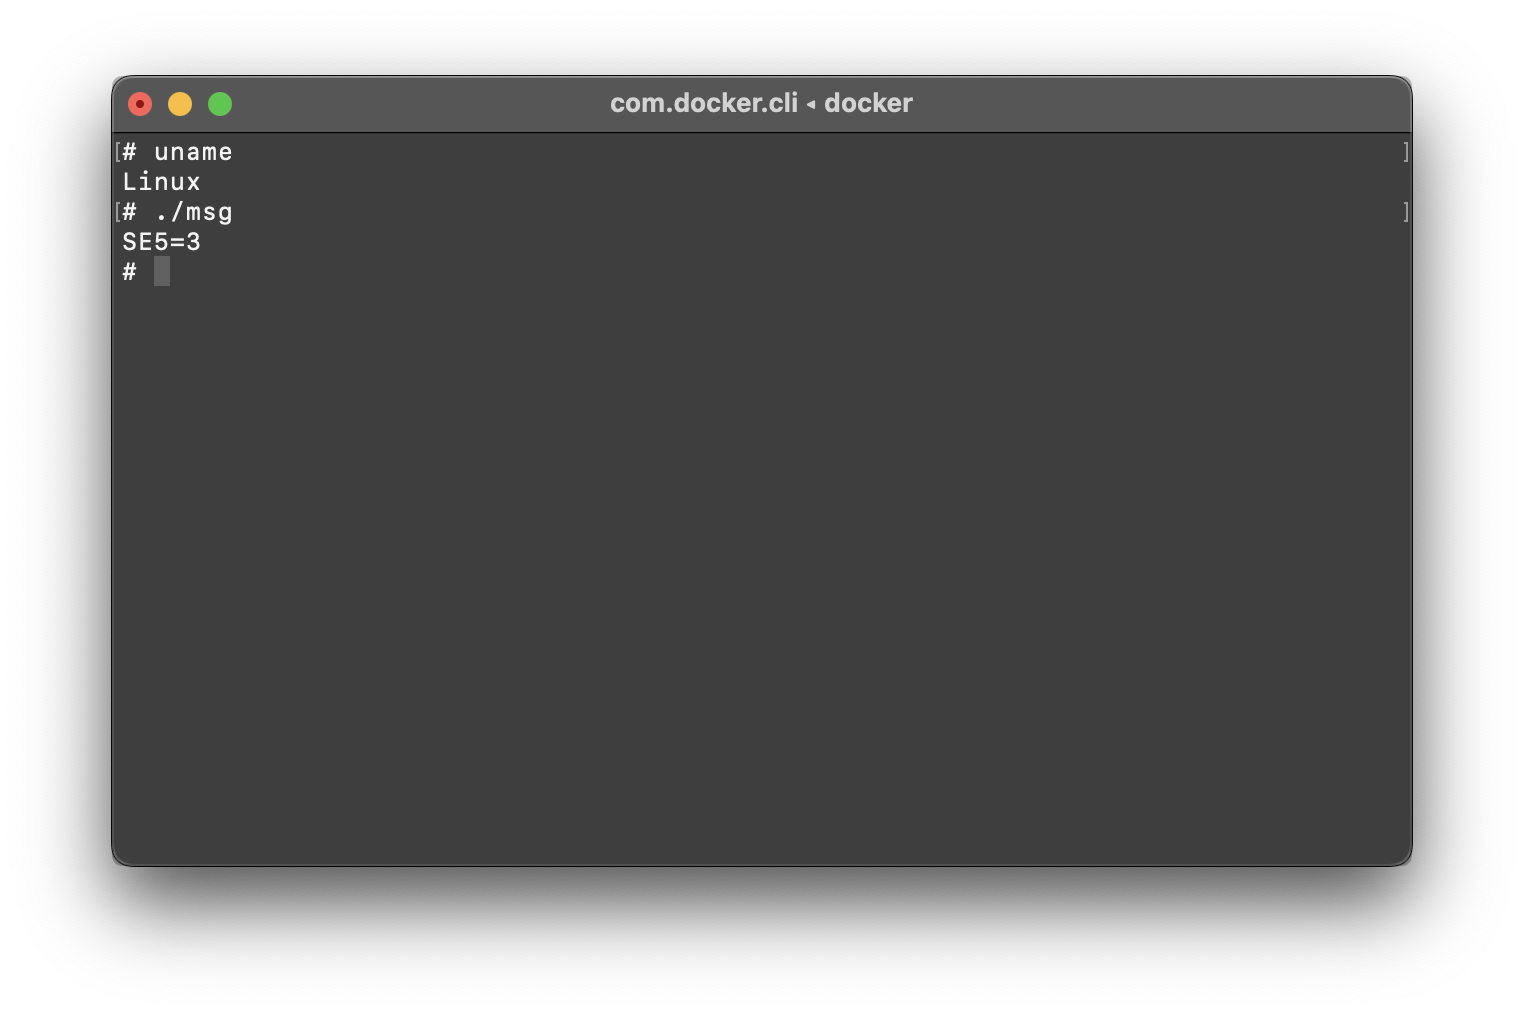
\includegraphics[width=\textwidth]{figure02.png}\vspace{-2em}
    \caption{Strings 2 \& 4 -- Linux \& SE5=3.}
    \label{fig:string2}
\end{figure}

% This assignment, part of the Reconnaissance and Vulnerability Identification\footnote{\href{https://learn.unm.edu/webapps/assignment/uploadAssignment?content_id=_7770481_1&course_id=_110809_1&user_id=_196414_1}{https://learn.unm.edu/webapps/assignment/uploadAssignment?content\_id=\_7770481\_1\&course\_id=\_110809\_1}} module, was designed to introduce students to the nmap scanning tool and to produce a detailed scan report for different hosts.

% \begin{tcolorbox}[colback=CrispBlue!5!white,colframe=CrispBlue!75!black,title=Output of \texttt{nmap -oN scanme-A.txt -A scanme.nmap.org}]\setstretch{1.25}

% \end{tcolorbox}



\end{document}